\documentclass[aspectratio=169, 10pt]{beamer}

% ---------- Tema y colores ----------
\usetheme{default}
\usecolortheme{default}
\setbeamertemplate{navigation symbols}{}
\setbeamertemplate{footline}[frame number]
\setbeamertemplate{frametitle continuation}{}

\definecolor{StanfordRed}{RGB}{140,21,21}
\definecolor{LightGray}{RGB}{240,240,240}
\definecolor{AccentGreen}{RGB}{0,130,100}
\definecolor{UCMBlue}{RGB}{4, 171, 226}
\definecolor{UCMNavy}{RGB}{20, 65, 134}

\definecolor{mitblue}{RGB}{20, 65, 134}
\definecolor{mitgray}{RGB}{169, 169, 169}

% Convenci\'on de colores: rojo = red que se entrena, azul = distribuci\'on fija / dato
\definecolor{AdaptRed}{RGB}{200, 40, 40}
\definecolor{FixedBlue}{RGB}{20, 65, 134}

\setbeamercolor{frametitle}{fg=white, bg=UCMBlue}
\setbeamercolor{title}{fg=white}
\setbeamercolor{author}{fg=white}
\setbeamercolor{institute}{fg=white!80}
\setbeamercolor{structure}{fg=UCMBlue}
\setbeamercolor{block title}{bg=UCMBlue!15!white, fg=UCMBlue}
\setbeamercolor{block body}{bg=LightGray}
\setbeamercolor{block title alerted}{bg=StanfordRed!15!white, fg=StanfordRed}
\setbeamercolor{block body alerted}{bg=LightGray}
\setbeamercolor{alerted text}{fg=UCMBlue}

\setbeamerfont{frametitle}{series=\bfseries, size=\large}
\setbeamerfont{title}{series=\bfseries, size=\LARGE}
\setbeamerfont{block title}{series=\bfseries}

% ---------- Paquetes ----------
\usepackage[utf8]{inputenc}
\usepackage[T1]{fontenc}
\usepackage[provide=*,spanish]{babel}
\usepackage{amsmath, amssymb}
\usepackage{graphicx}
\usepackage{tikz}
\usepackage{pgfplots}
\pgfplotsset{compat=1.18}
\usetikzlibrary{arrows, arrows.meta, shapes, shapes.geometric, positioning,
	fit, calc, matrix, chains, mindmap, decorations.pathreplacing,
	backgrounds, shadows, patterns}
\usepackage{booktabs}
\usepackage{xcolor}
\usepackage{multicol}
\usepackage{tcolorbox}
\tcbuselibrary{skins, breakable}
\usepackage{fontawesome5}

% ---------- Comandos \'utiles ----------
\providecommand{\R}{\mathbb{R}}
\providecommand{\E}{\mathbb{E}}
\newcommand{\KL}{\mathrm{KL}}
\newcommand{\pdata}{p_{\text{data}}}
\newcommand{\ad}[1]{{\color{AdaptRed}#1}}
\newcommand{\fx}[1]{{\color{FixedBlue}#1}}
\newcommand{\good}{{\color{AccentGreen}\faCheck}}
\newcommand{\bad}{{\color{AdaptRed}\faTimes}}
\newcommand{\meh}{{\color{orange}\faMinus}}

\newcommand{\formula}[1]{%
	\begin{tcolorbox}[colback=UCMBlue!8, colframe=UCMBlue, arc=4pt,
		boxsep=2pt, left=6pt, right=6pt, top=3pt, bottom=3pt]
		#1
	\end{tcolorbox}
}

% ---------- Portada ----------
\title{\textbf{Modelos Generativos Profundos}}
\subtitle{Autoencoders variacionales, flujos normalizantes, GANs y modelos basados en energ\'ia}
\author{Sergio Hern\'andez, PhD\\ shernandez@ucm.cl}
\institute{
	\begin{tikzpicture}[scale=0.42, every node/.style={transform shape}]
		\foreach \i/\y in {1/0,2/1,3/2}{\node[circle,draw=white,fill=white!20,minimum size=4mm] (i\i) at (0,\y){};}
		\foreach \i/\y in {1/-0.5,2/0.5,3/1.5,4/2.5}{\node[circle,draw=white,fill=white!35,minimum size=4mm] (h\i) at (2,\y){};}
		\foreach \i/\y in {1/0.5,2/1.5}{\node[circle,draw=white,fill=white!50,minimum size=4mm] (o\i) at (4,\y){};}
		\foreach \a in {1,2,3}\foreach \b in {1,2,3,4}{\draw[white,opacity=0.5] (i\a)--(h\b);}
		\foreach \a in {1,2,3,4}\foreach \b in {1,2}{\draw[white,opacity=0.5] (h\a)--(o\b);}
	\end{tikzpicture}
	\\ \textbf{Mag\'ister en Data Science --- Universidad Cat\'olica del Maule}}
\date{}

\begin{document}
% --- T\'itulo ---
{
	\setbeamertemplate{background}{
		
\begin{tikzpicture}[remember picture, overlay]
			\fill[UCMBlue] (current page.south west) rectangle (current page.north east);
			\fill[UCMBlue!70!black, opacity=0.5]
			(current page.south west) -- ++(0,3) -- ++(18,0) -- cycle;
			\foreach \i in {1,...,40}{
				\fill[white, opacity=0.04]
				({random()*17}, {random()*10}) circle ({random()*0.3});
			}
		\end{tikzpicture}
	}
	\begin{frame}[plain]
		\vspace{1.2cm}
		\titlepage
		\begin{tikzpicture}[remember picture, overlay]
			\node[white, opacity=0.15, font=\fontsize{80}{80}\selectfont]
			at (current page.east) [xshift=-2.4cm] {$p_\theta$};
		\end{tikzpicture}
	\end{frame}
}

% =================================================================
\section{Introducci\'on}

\begin{frame}[shrink]{Discriminativo vs.\ Generativo}

	\begin{columns}[T]
		\begin{column}{0.5\textwidth}
			\begin{block}{Modelo Discriminativo}
				\begin{itemize}
					\item Aprende $p(y \mid x)$: una frontera de decisi\'on.
					\item Clasificaci\'on, detecci\'on, segmentaci\'on (clases 2.1--2.6).
					\item No sabe ``c\'omo se ve'' un dato.
				\end{itemize}
			\end{block}
		\end{column}

		\begin{column}{0.5\textwidth}
			\begin{block}{Modelo Generativo}
				\begin{itemize}
					\item Aprende $p(x)$ (o $p(x \mid y)$): la distribuci\'on de los datos.
					\item Permite \textbf{muestrear} datos nuevos $x \sim p_\theta$.
					\item Permite \textbf{evaluar} qu\'e tan probable es un $x$.
				\end{itemize}
			\end{block}
		\end{column}
	\end{columns}

	\vspace{0.3cm}

	\begin{center}
		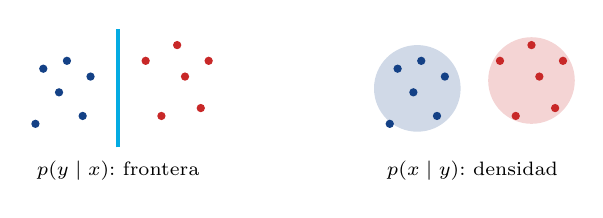
\begin{tikzpicture}
			\begin{scope}
				\foreach \x/\y in {0.2/0.3,0.5/0.7,0.3/1.0,0.8/0.4,0.6/1.1,0.9/0.9}{\fill[FixedBlue] (\x,\y) circle (1.5pt);}
				\foreach \x/\y in {1.8/0.4,2.1/0.9,1.6/1.1,2.3/0.5,2.0/1.3,2.4/1.1}{\fill[AdaptRed] (\x,\y) circle (1.5pt);}
				\draw[very thick, UCMBlue] (1.25,0) -- (1.25,1.5);
				\node[font=\scriptsize] at (1.25,-0.3) {$p(y\mid x)$: frontera};
			\end{scope}
			\begin{scope}[shift={(4.5,0)}]
				\fill[FixedBlue!20] (0.55,0.75) ellipse (0.55 and 0.55);
				\fill[AdaptRed!20] (2.0,0.85) ellipse (0.55 and 0.55);
				\foreach \x/\y in {0.2/0.3,0.5/0.7,0.3/1.0,0.8/0.4,0.6/1.1,0.9/0.9}{\fill[FixedBlue] (\x,\y) circle (1.5pt);}
				\foreach \x/\y in {1.8/0.4,2.1/0.9,1.6/1.1,2.3/0.5,2.0/1.3,2.4/1.1}{\fill[AdaptRed] (\x,\y) circle (1.5pt);}
				\node[font=\scriptsize] at (1.25,-0.3) {$p(x\mid y)$: densidad};
			\end{scope}
		\end{tikzpicture}
	\end{center}

	\begin{alertblock}{Idea Central}
		Un modelo generativo $p_\theta(x)$ debe asignar \textbf{alta probabilidad} a datos reales y \textbf{baja} a todo lo dem\'as, en espacios de alt\'isima dimensi\'on (una imagen $256 \times 256 \times 3$ vive en $\R^{196\,608}$).
	\end{alertblock}

\end{frame}

\begin{frame}{¿Para Qu\'e Sirve un Modelo Generativo?}

	\begin{columns}[T]
		\begin{column}{0.33\textwidth}
			\begin{block}{Muestrear}
				\small
				\begin{itemize}
					\item S\'intesis de im\'agenes, audio, texto.
					\item Datos sint\'eticos para entrenar (clase 2.5).
					\item Aumentaci\'on de datos m\'edicos escasos.
				\end{itemize}
			\end{block}
		\end{column}

		\begin{column}{0.33\textwidth}
			\begin{block}{Evaluar $p_\theta(x)$}
				\small
				\begin{itemize}
					\item Detecci\'on de anomal\'ias: $p_\theta(x)$ bajo $\Rightarrow$ at\'ipico.
					\item Compresi\'on (Shannon: $-\log_2 p(x)$ bits).
					\item Comparar modelos (log-verosimilitud).
				\end{itemize}
			\end{block}
		\end{column}

		\begin{column}{0.33\textwidth}
			\begin{block}{Representar}
				\small
				\begin{itemize}
					\item Variables latentes $z$ como \textbf{representaci\'on} compacta.
					\item Interpolaci\'on y edici\'on sem\'antica.
					\item Semi-supervisado, aprendizaje de features.
				\end{itemize}
			\end{block}
		\end{column}
	\end{columns}

	\vspace{0.4cm}

	\begin{block}{Hoy}
		Cuatro familias que resuelven el mismo problema con distintos compromisos:
		\textbf{VAE} (verosimilitud aproximada), \textbf{flujos normalizantes} (verosimilitud exacta),
		\textbf{GAN} (impl\'icito, adversario) y \textbf{modelos basados en energ\'ia} (densidad no normalizada).
	\end{block}

\end{frame}

\begin{frame}[shrink]{M\'axima Verosimilitud = Minimizar KL}

	Dado $\mathcal{D} = \{x^{(i)}\}_{i=1}^N \sim \pdata$, buscamos $\theta$ tal que $p_\theta \approx \pdata$.

	\formula{
		\[
		\theta^* = \arg\max_\theta \frac{1}{N}\sum_{i=1}^N \log p_\theta(x^{(i)})
		\;\xrightarrow{N\to\infty}\;
		\arg\max_\theta \E_{\pdata}\big[\log p_\theta(x)\big]
		= \arg\min_\theta \KL\big(\pdata \,\|\, p_\theta\big)
		\]
	}

	\begin{columns}[T]
		\begin{column}{0.5\textwidth}
			\begin{block}{Por qu\'e}
				\small
				\[
				\KL(\pdata\|p_\theta) = \underbrace{\E_{\pdata}[\log \pdata]}_{\text{no depende de }\theta} - \E_{\pdata}[\log p_\theta]
				\]
			\end{block}
		\end{column}

		\begin{column}{0.5\textwidth}
			\begin{block}{Dos requisitos que chocan}
				\small
				\begin{enumerate}
					\item $p_\theta$ \textbf{flexible}: redes profundas.
					\item $p_\theta$ \textbf{normalizada}: $\int p_\theta(x)\,dx = 1$.
				\end{enumerate}
				Una red arbitraria $f_\theta(x) \ge 0$ no integra 1.
			\end{block}
		\end{column}
	\end{columns}

	\vspace{0.2cm}

	\begin{alertblock}{El Problema Central}
		Cada familia de modelos generativos es, en el fondo, una \textbf{estrategia distinta para lidiar con la normalizaci\'on}.
	\end{alertblock}

\end{frame}

\begin{frame}{Taxonom\'ia de Modelos Generativos Profundos}

	\begin{center}
		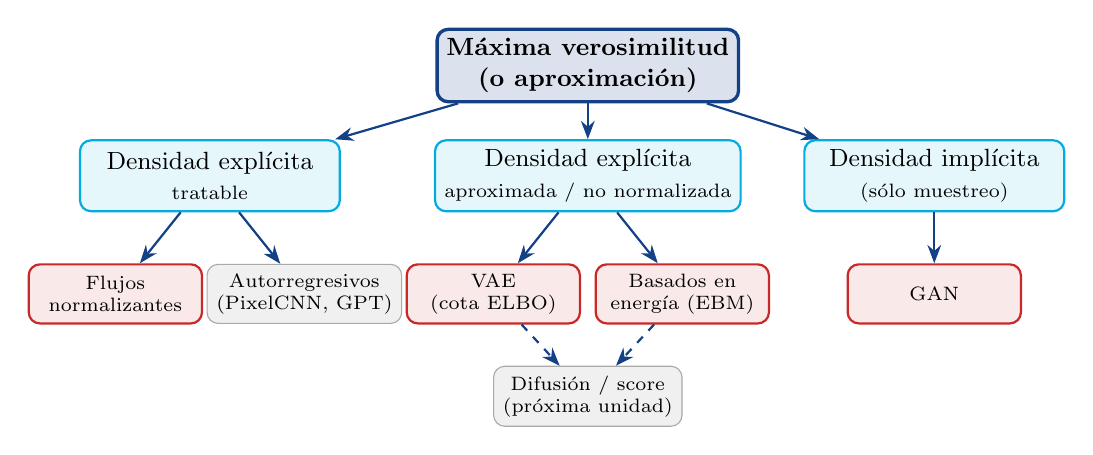
\begin{tikzpicture}[
				root/.style={draw=UCMNavy, very thick, fill=UCMNavy!15, rounded corners, align=center, font=\small\bfseries, minimum width=3cm},
				cat/.style={draw=UCMBlue, thick, fill=UCMBlue!10, rounded corners, align=center, font=\small, minimum width=3.3cm, minimum height=0.9cm},
				leaf/.style={draw=mitgray, fill=LightGray, rounded corners, align=center, font=\scriptsize, minimum width=2.2cm, minimum height=0.75cm},
				hot/.style={draw=AdaptRed, thick, fill=AdaptRed!10, rounded corners, align=center, font=\scriptsize, minimum width=2.2cm, minimum height=0.75cm},
				arr/.style={-Stealth, thick, UCMNavy}]
			\node[root] (r) at (0,0) {M\'axima verosimilitud\\ (o aproximaci\'on)};
			\node[cat] (e) at (-4.8,-1.4) {Densidad expl\'icita\\ \scriptsize tratable};
			\node[cat] (a) at (0,-1.4) {Densidad expl\'icita\\ \scriptsize aproximada / no normalizada};
			\node[cat] (i) at (4.4,-1.4) {Densidad impl\'icita\\ \scriptsize (s\'olo muestreo)};

			\node[hot]  (nf) at (-6.0,-2.9) {Flujos\\ normalizantes};
			\node[leaf] (ar) at (-3.6,-2.9) {Autorregresivos\\ (PixelCNN, GPT)};
			\node[hot]  (vae) at (-1.2,-2.9) {VAE\\ (cota ELBO)};
			\node[hot]  (ebm) at (1.2,-2.9) {Basados en\\ energ\'ia (EBM)};
			\node[hot]  (gan) at (4.4,-2.9) {GAN};

			\node[leaf] (dif) at (0,-4.2) {Difusi\'on / score\\ (pr\'oxima unidad)};

			\draw[arr] (r) -- (e); \draw[arr] (r) -- (a); \draw[arr] (r) -- (i);
			\draw[arr] (e) -- (nf); \draw[arr] (e) -- (ar);
			\draw[arr] (a) -- (vae); \draw[arr] (a) -- (ebm);
			\draw[arr] (i) -- (gan);
			\draw[arr, dashed] (vae) -- (dif); \draw[arr, dashed] (ebm) -- (dif);
		\end{tikzpicture}
	\end{center}

	\small En \ad{rojo}: lo que veremos hoy. La difusi\'on combina ideas del VAE (variable latente jer\'arquica) y de los EBM (score $\nabla_x \log p$).

\end{frame}

% =================================================================
\section{Autoencoders}

\begin{frame}[shrink]{Autoencoder: Comprimir y Reconstruir}

	\begin{center}
		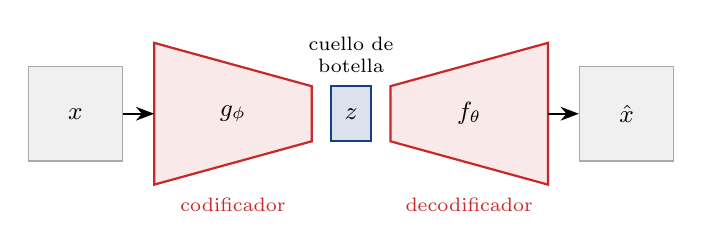
\begin{tikzpicture}[
				arr/.style={-Stealth, thick}]
			\node[draw=mitgray, fill=LightGray, minimum width=1.2cm, minimum height=1.2cm, font=\small] (x) at (0,0) {$x$};
			\draw[thick, draw=AdaptRed, fill=AdaptRed!10] (1.0,0.9) -- (3.0,0.35) -- (3.0,-0.35) -- (1.0,-0.9) -- cycle;
			\node[font=\small] at (2.0,0) {$g_\phi$};
			\node[font=\scriptsize, AdaptRed] at (2.0,-1.15) {codificador};
			\node[draw=UCMNavy, thick, fill=UCMNavy!15, minimum width=0.5cm, minimum height=0.7cm, font=\small] (z) at (3.5,0) {$z$};
			\draw[thick, draw=AdaptRed, fill=AdaptRed!10] (4.0,0.35) -- (6.0,0.9) -- (6.0,-0.9) -- (4.0,-0.35) -- cycle;
			\node[font=\small] at (5.0,0) {$f_\theta$};
			\node[font=\scriptsize, AdaptRed] at (5.0,-1.15) {decodificador};
			\node[draw=mitgray, fill=LightGray, minimum width=1.2cm, minimum height=1.2cm, font=\small] (xh) at (7.0,0) {$\hat x$};
			\draw[arr] (x) -- (1.0,0); \draw[arr] (6.0,0) -- (xh);
			\node[font=\scriptsize, align=center] at (3.5,0.75) {cuello de\\ botella};
		\end{tikzpicture}
	\end{center}

	\formula{
		\[
		\phi^*, \theta^* = \arg\min_{\phi,\theta} \frac{1}{N}\sum_{i=1}^N \big\| x^{(i)} - f_\theta\big(g_\phi(x^{(i)})\big)\big\|^2,
		\qquad z = g_\phi(x) \in \R^{d},\; d \ll D
		\]
	}

	\begin{columns}[T]
		\begin{column}{0.5\textwidth}
			\begin{block}{Qu\'e aprende}
				\small
				\begin{itemize}
					\item Con $f,g$ lineales: equivale a \textbf{PCA}.
					\item No lineal: una variedad (\textit{manifold}) de baja dimensi\'on.
					\item Usos: compresi\'on, denoising, anomal\'ias.
				\end{itemize}
			\end{block}
		\end{column}

		\begin{column}{0.5\textwidth}
			\begin{alertblock}{¿Es un modelo generativo?}
				\small
				\textbf{No todav\'ia.} Si muestreamos $z$ al azar y decodificamos, $f_\theta(z)$ suele ser basura: el espacio latente tiene ``huecos'' y no sabemos \textbf{de qu\'e distribuci\'on} sacar $z$.
			\end{alertblock}
		\end{column}
	\end{columns}

\end{frame}

\begin{frame}{El Espacio Latente de un Autoencoder}

	\begin{columns}[c]
		\begin{column}{0.48\textwidth}
			\begin{center}
				\begin{tikzpicture}[scale=0.9]
					\draw[-Stealth] (-0.2,0) -- (4.2,0) node[right, font=\scriptsize] {$z_1$};
					\draw[-Stealth] (0,-0.2) -- (0,3.4) node[above, font=\scriptsize] {$z_2$};
					\foreach \x/\y in {0.5/0.5,0.7/0.8,0.6/0.4,0.9/0.6,0.4/0.7}{\fill[FixedBlue] (\x,\y) circle (1.6pt);}
					\foreach \x/\y in {3.2/0.6,3.5/0.9,3.4/0.4,3.7/0.7}{\fill[AdaptRed] (\x,\y) circle (1.6pt);}
					\foreach \x/\y in {1.5/2.8,1.8/3.0,1.6/2.5,2.0/2.7}{\fill[AccentGreen] (\x,\y) circle (1.6pt);}
					\foreach \x/\y in {3.6/2.9,3.9/3.1}{\fill[orange] (\x,\y) circle (1.6pt);}
					\node[draw=black, thick, cross out, minimum size=5pt, inner sep=0pt] at (2.1,1.4) {};
					\node[font=\scriptsize, align=center] at (2.4,1.0) {$z$ al azar\\ $\Rightarrow$ ?};
				\end{tikzpicture}
			\end{center}
			\scriptsize Autoencoder determinista: c\'odigos dispersos, regiones vac\'ias, escala arbitraria.
		\end{column}

		\begin{column}{0.48\textwidth}
			\begin{center}
				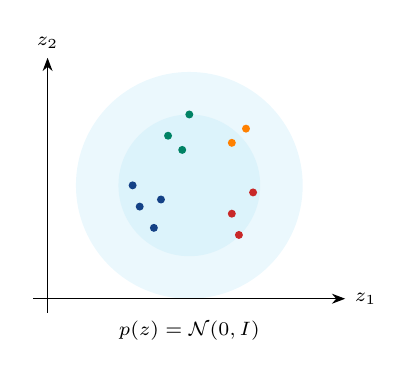
\begin{tikzpicture}[scale=0.9]
					\fill[UCMBlue!8] (2,1.6) circle (1.6);
					\fill[UCMBlue!14] (2,1.6) circle (1.0);
					\draw[-Stealth] (-0.2,0) -- (4.2,0) node[right, font=\scriptsize] {$z_1$};
					\draw[-Stealth] (0,-0.2) -- (0,3.4) node[above, font=\scriptsize] {$z_2$};
					\foreach \x/\y in {1.3/1.3,1.5/1.0,1.2/1.6,1.6/1.4}{\fill[FixedBlue] (\x,\y) circle (1.6pt);}
					\foreach \x/\y in {2.6/1.2,2.9/1.5,2.7/0.9}{\fill[AdaptRed] (\x,\y) circle (1.6pt);}
					\foreach \x/\y in {1.7/2.3,2.0/2.6,1.9/2.1}{\fill[AccentGreen] (\x,\y) circle (1.6pt);}
					\foreach \x/\y in {2.6/2.2,2.8/2.4}{\fill[orange] (\x,\y) circle (1.6pt);}
					\node[font=\scriptsize] at (2,-0.45) {$p(z) = \mathcal{N}(0, I)$};
				\end{tikzpicture}
			\end{center}
			\scriptsize VAE: los c\'odigos se fuerzan a cubrir una distribuci\'on conocida $\Rightarrow$ podemos muestrear $z \sim p(z)$.
		\end{column}
	\end{columns}

	\vspace{0.3cm}

	\begin{block}{Lo que falta}
		Un \textbf{modelo probabil\'istico} expl\'icito: una distribuci\'on a priori $p(z)$ f\'acil de muestrear y una verosimilitud $p_\theta(x\mid z)$. Eso es el \textbf{autoencoder variacional}.
	\end{block}

\end{frame}

% =================================================================
\section{Autoencoders Variacionales}

\begin{frame}{Modelo de Variable Latente}

	\begin{columns}[c]
		\begin{column}{0.35\textwidth}
			\begin{center}
				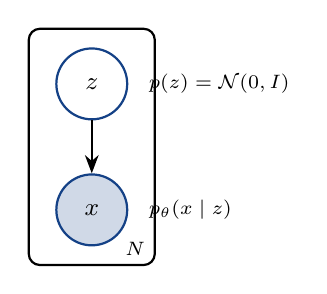
\begin{tikzpicture}[
						rv/.style={circle, draw=UCMNavy, thick, minimum size=0.9cm, font=\small},
						obs/.style={circle, draw=UCMNavy, thick, fill=UCMNavy!20, minimum size=0.9cm, font=\small}]
					\node[rv] (z) at (0,1.6) {$z$};
					\node[obs] (x) at (0,0) {$x$};
					\draw[-Stealth, thick] (z) -- (x);
					\node[font=\scriptsize, anchor=west] at (0.6,1.6) {$p(z)=\mathcal{N}(0,I)$};
					\node[font=\scriptsize, anchor=west] at (0.6,0) {$p_\theta(x\mid z)$};
					\draw[thick, rounded corners] (-0.8,-0.7) rectangle (0.8,2.3);
					\node[font=\scriptsize] at (0.55,-0.5) {$N$};
				\end{tikzpicture}
			\end{center}
		\end{column}

		\begin{column}{0.63\textwidth}
			\begin{block}{Proceso generativo}
				\begin{enumerate}
					\item $z \sim p(z) = \mathcal{N}(0, I_d)$
					\item $x \sim p_\theta(x \mid z) = \mathcal{N}\big(x;\, \ad{f_\theta(z)},\, \sigma^2 I\big)$ \\
					      {\small (o Bernoulli para im\'agenes binarias)}
				\end{enumerate}
				$\ad{f_\theta}$ es una red neuronal: el \textbf{decodificador}.
			\end{block}
		\end{column}
	\end{columns}

	\vspace{0.3cm}

	\formula{
		\[
		p_\theta(x) = \int p_\theta(x \mid z)\, p(z)\, dz
		\qquad\text{(mezcla infinita de gaussianas)}
		\]
	}

	\begin{alertblock}{Problema}
		La integral es \textbf{intratable}: $f_\theta$ es no lineal y $z$ tiene decenas o cientos de dimensiones. Tampoco podemos calcular el posterior $p_\theta(z\mid x) = p_\theta(x\mid z)p(z)/p_\theta(x)$, que necesitar\'iamos para EM.
	\end{alertblock}

\end{frame}

\begin{frame}[shrink]{¿Por Qu\'e no Monte Carlo Ingenuo?}

	\formula{
		\[
		p_\theta(x) = \E_{z\sim p(z)}\big[p_\theta(x \mid z)\big] \approx \frac{1}{S}\sum_{s=1}^S p_\theta(x \mid z^{(s)}), \qquad z^{(s)} \sim \mathcal{N}(0, I)
		\]
	}

	\begin{columns}[c]
		\begin{column}{0.5\textwidth}
			\begin{center}
				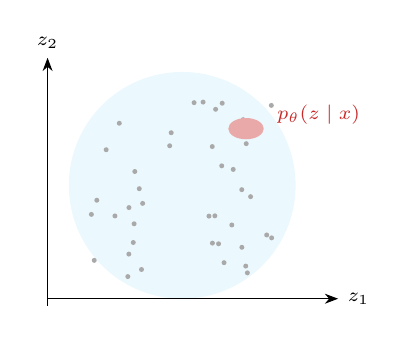
\begin{tikzpicture}[scale=0.9]
					\fill[UCMBlue!8] (2,1.6) circle (1.6);
					\draw[-Stealth] (0.1,0) -- (4.2,0) node[right, font=\scriptsize] {$z_1$};
					\draw[-Stealth] (0.1,-0.1) -- (0.1,3.4) node[above, font=\scriptsize] {$z_2$};
					\foreach \i in {1,...,40}{\fill[mitgray] ({2+1.3*rand},{1.6+1.3*rand}) circle (1pt);}
					\fill[AdaptRed!40] (2.9,2.4) ellipse (0.25 and 0.15);
					\node[font=\scriptsize, AdaptRed, anchor=west] at (3.2,2.6) {$p_\theta(z\mid x)$};
				\end{tikzpicture}
			\end{center}
		\end{column}

		\begin{column}{0.5\textwidth}
			\begin{block}{El problema}
				\small
				\begin{itemize}
					\item Para un $x$ dado, s\'olo una regi\'on \textbf{diminuta} de $z$ explica $x$ (en \ad{rojo}).
					\item Casi todas las muestras del prior dan $p_\theta(x\mid z) \approx 0$.
					\item Varianza enorme; $S$ crece exponencialmente con $d$.
				\end{itemize}
			\end{block}
		\end{column}
	\end{columns}

	\vspace{0.3cm}

	\begin{block}{Idea}
		Usar una distribuci\'on auxiliar $\ad{q_\phi(z\mid x)}$ que proponga $z$ \textbf{plausibles para cada $x$}: el \textbf{codificador}. Esto es \textbf{inferencia variacional} (como en los modelos gr\'aficos probabil\'isticos), pero \textit{amortizada} por una red.
	\end{block}

\end{frame}

\begin{frame}{La Cota Inferior de la Evidencia (ELBO)}

	Para cualquier $q_\phi(z\mid x)$, usando la desigualdad de Jensen:
	\[
	\log p_\theta(x) = \log \E_{q_\phi(z\mid x)}\!\left[\frac{p_\theta(x, z)}{q_\phi(z\mid x)}\right]
	\;\ge\; \E_{q_\phi(z\mid x)}\!\left[\log \frac{p_\theta(x, z)}{q_\phi(z\mid x)}\right] \equiv \mathcal{L}(\theta,\phi; x)
	\]

	\vspace{-0.1cm}

	\formula{
		\[
		\log p_\theta(x) = \underbrace{\mathcal{L}(\theta,\phi;x)}_{\text{ELBO}} + \underbrace{\KL\big(q_\phi(z\mid x)\,\|\,p_\theta(z\mid x)\big)}_{\ge 0}
		\]
	}

	\begin{columns}[T]
		\begin{column}{0.5\textwidth}
			\begin{block}{Lectura}
				\small
				\begin{itemize}
					\item La brecha es exactamente el KL entre la aproximaci\'on y el posterior verdadero.
					\item Maximizar en $\phi$ $\Rightarrow$ $q_\phi$ se acerca al posterior.
					\item Maximizar en $\theta$ $\Rightarrow$ sube la verosimilitud.
				\end{itemize}
			\end{block}
		\end{column}

		\begin{column}{0.5\textwidth}
			\begin{center}
				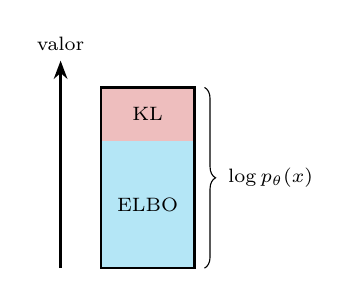
\begin{tikzpicture}[scale=0.85]
					\draw[thick, -Stealth] (0,0) -- (0,3.1) node[above, font=\scriptsize] {valor};
					\fill[UCMBlue!30] (0.6,0) rectangle (2.0,1.9);
					\fill[AdaptRed!30] (0.6,1.9) rectangle (2.0,2.7);
					\draw[thick] (0.6,0) rectangle (2.0,2.7);
					\node[font=\scriptsize] at (1.3,0.95) {ELBO};
					\node[font=\scriptsize] at (1.3,2.3) {KL};
					\draw[decorate, decoration={brace, amplitude=4pt}] (2.15,2.7) -- (2.15,0) node[midway, right=5pt, font=\scriptsize] {$\log p_\theta(x)$};
				\end{tikzpicture}
			\end{center}
		\end{column}
	\end{columns}

\end{frame}

\begin{frame}[shrink]{El ELBO como Reconstrucci\'on + Regularizaci\'on}

	Reescribiendo $p_\theta(x,z) = p_\theta(x\mid z)\,p(z)$:

	\formula{
		\[
		\mathcal{L}(\theta,\phi;x) =
		\underbrace{\E_{q_\phi(z\mid x)}\big[\log p_\theta(x \mid z)\big]}_{\text{reconstrucci\'on}}
		\;-\;
		\underbrace{\KL\big(q_\phi(z\mid x)\,\|\,p(z)\big)}_{\text{regularizaci\'on}}
		\]
	}

	\begin{columns}[T]
		\begin{column}{0.5\textwidth}
			\begin{block}{T\'ermino de reconstrucci\'on}
				\small
				\begin{itemize}
					\item Con $p_\theta(x\mid z) = \mathcal{N}(f_\theta(z), \sigma^2 I)$:
					\[
					\log p_\theta(x\mid z) = -\tfrac{1}{2\sigma^2}\|x - f_\theta(z)\|^2 + \text{cte}
					\]
					\item Es el \textbf{error cuadr\'atico} del autoencoder.
					\item Bernoulli $\Rightarrow$ entrop\'ia cruzada binaria.
				\end{itemize}
			\end{block}
		\end{column}

		\begin{column}{0.5\textwidth}
			\begin{block}{T\'ermino KL}
				\small
				\begin{itemize}
					\item Empuja cada $q_\phi(z\mid x)$ hacia el prior $\mathcal{N}(0,I)$.
					\item Rellena los ``huecos'' del espacio latente.
					\item Penaliza c\'odigos que memorizan cada $x$.
				\end{itemize}
			\end{block}
		\end{column}
	\end{columns}

	\vspace{0.2cm}

	\begin{alertblock}{Compromiso}
		Reconstruir bien pide codificar mucha informaci\'on de $x$ en $z$; el KL pide que $z$ no se aleje del prior. El VAE equilibra \textbf{fidelidad} y \textbf{regularidad} del espacio latente.
	\end{alertblock}

\end{frame}

\begin{frame}{Codificador Gaussiano y KL en Forma Cerrada}

	Elegimos un codificador gaussiano diagonal:

	\formula{
		\[
		q_\phi(z\mid x) = \mathcal{N}\big(z;\; \ad{\mu_\phi(x)},\; \mathrm{diag}(\ad{\sigma^2_\phi(x)})\big)
		\]
	}

	La red $g_\phi$ devuelve dos vectores: $\mu_\phi(x) \in \R^d$ y $\log \sigma^2_\phi(x) \in \R^d$ (el logaritmo garantiza $\sigma^2 > 0$).

	\vspace{0.2cm}

	\begin{block}{KL entre dos gaussianas (por dimensi\'on)}
		\[
		\KL\big(\mathcal{N}(\mu, \sigma^2)\,\|\,\mathcal{N}(0,1)\big)
		= \frac{1}{2}\Big(\mu^2 + \sigma^2 - \log \sigma^2 - 1\Big)
		\]
		\[
		\Rightarrow\quad
		\KL\big(q_\phi(z\mid x)\,\|\,p(z)\big) = \frac{1}{2}\sum_{j=1}^{d}\Big(\mu_j^2 + \sigma_j^2 - \log\sigma_j^2 - 1\Big)
		\]
	\end{block}

	\vspace{0.1cm}

	\small El KL se calcula \textbf{exactamente}; s\'olo el t\'ermino de reconstrucci\'on necesita Monte Carlo (en la pr\'actica, basta $S=1$ muestra por dato).

\end{frame}

\begin{frame}[shrink]{El Truco de Reparametrizaci\'on}

	\textbf{Problema:} necesitamos $\nabla_\phi \E_{q_\phi(z\mid x)}[\log p_\theta(x\mid z)]$, pero el muestreo $z \sim q_\phi$ \textbf{no es diferenciable} respecto a $\phi$.

	\vspace{0.2cm}

	\begin{columns}[c]
		\begin{column}{0.5\textwidth}
			\begin{center}
				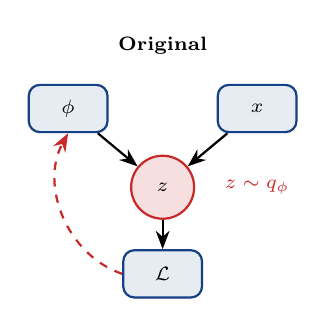
\begin{tikzpicture}[
						det/.style={draw=UCMNavy, thick, fill=UCMNavy!10, rounded corners, minimum width=1.0cm, minimum height=0.6cm, font=\scriptsize},
						sto/.style={draw=AdaptRed, thick, fill=AdaptRed!15, circle, minimum size=0.8cm, font=\scriptsize},
						arr/.style={-Stealth, thick}]
					\node[font=\scriptsize\bfseries] at (1.2,2.6) {Original};
					\node[det] (phi) at (0,1.8) {$\phi$};
					\node[det] (x) at (2.4,1.8) {$x$};
					\node[sto] (z) at (1.2,0.8) {$z$};
					\node[det] (f) at (1.2,-0.3) {$\mathcal{L}$};
					\draw[arr] (phi) -- (z); \draw[arr] (x) -- (z); \draw[arr] (z) -- (f);
					\draw[arr, dashed, AdaptRed] (f.west) to[bend left=50] node[left, font=\scriptsize] {\bad} (phi.south);
					\node[font=\scriptsize, AdaptRed] at (2.4,0.8) {$z \sim q_\phi$};
				\end{tikzpicture}
			\end{center}
		\end{column}

		\begin{column}{0.5\textwidth}
			\begin{center}
				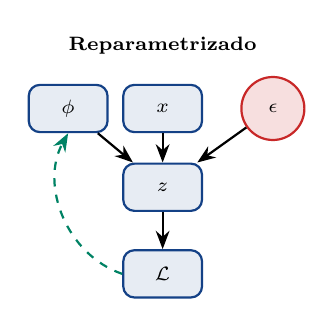
\begin{tikzpicture}[
						det/.style={draw=UCMNavy, thick, fill=UCMNavy!10, rounded corners, minimum width=1.0cm, minimum height=0.6cm, font=\scriptsize},
						sto/.style={draw=AdaptRed, thick, fill=AdaptRed!15, circle, minimum size=0.8cm, font=\scriptsize},
						arr/.style={-Stealth, thick}]
					\node[font=\scriptsize\bfseries] at (1.2,2.6) {Reparametrizado};
					\node[det] (phi) at (0,1.8) {$\phi$};
					\node[det] (x) at (1.2,1.8) {$x$};
					\node[sto] (eps) at (2.6,1.8) {$\epsilon$};
					\node[det] (z) at (1.2,0.8) {$z$};
					\node[det] (f) at (1.2,-0.3) {$\mathcal{L}$};
					\draw[arr] (phi) -- (z); \draw[arr] (x) -- (z); \draw[arr] (eps) -- (z); \draw[arr] (z) -- (f);
					\draw[arr, dashed, AccentGreen] (f.west) to[bend left=50] node[left, font=\scriptsize] {\good} (phi.south);
				\end{tikzpicture}
			\end{center}
		\end{column}
	\end{columns}

	\formula{
		\[
		z = \mu_\phi(x) + \sigma_\phi(x) \odot \epsilon, \qquad \epsilon \sim \mathcal{N}(0, I)
		\quad\Longrightarrow\quad
		\nabla_\phi \E_{q_\phi}\big[h(z)\big] = \E_{\epsilon}\Big[\nabla_\phi\, h\big(\mu_\phi(x) + \sigma_\phi(x)\odot\epsilon\big)\Big]
		\]
	}

	\small La aleatoriedad se traslada a una variable $\epsilon$ que \textbf{no depende de $\phi$}: el gradiente pasa por $\mu$ y $\sigma$ con backpropagation est\'andar.

\end{frame}

\begin{frame}{Arquitectura Completa del VAE}

	\begin{center}
		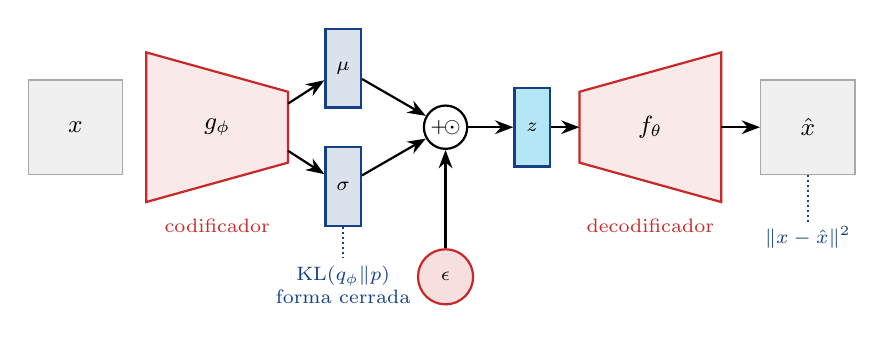
\begin{tikzpicture}[
				arr/.style={-Stealth, thick},
				vec/.style={draw=UCMNavy, thick, fill=UCMNavy!15, minimum width=0.45cm, minimum height=1.0cm, font=\scriptsize}]
			\node[draw=mitgray, fill=LightGray, minimum width=1.2cm, minimum height=1.2cm, font=\small] (x) at (0,0) {$x$};
			\draw[thick, draw=AdaptRed, fill=AdaptRed!10] (0.9,0.95) -- (2.7,0.45) -- (2.7,-0.45) -- (0.9,-0.95) -- cycle;
			\node[font=\small] at (1.8,0) {$g_\phi$};
			\node[vec] (mu) at (3.4,0.75) {$\mu$};
			\node[vec] (sig) at (3.4,-0.75) {$\sigma$};
			\node[circle, draw=AdaptRed, thick, fill=AdaptRed!15, minimum size=0.7cm, font=\scriptsize] (eps) at (4.7,-1.9) {$\epsilon$};
			\node[circle, draw=black, thick, minimum size=0.55cm, font=\scriptsize, inner sep=0pt] (op) at (4.7,0) {$+\!\odot$};
			\node[vec, fill=UCMBlue!30] (z) at (5.8,0) {$z$};
			\draw[thick, draw=AdaptRed, fill=AdaptRed!10] (6.4,0.45) -- (8.2,0.95) -- (8.2,-0.95) -- (6.4,-0.45) -- cycle;
			\node[font=\small] at (7.3,0) {$f_\theta$};
			\node[draw=mitgray, fill=LightGray, minimum width=1.2cm, minimum height=1.2cm, font=\small] (xh) at (9.3,0) {$\hat x$};

			\draw[arr] (2.7,0.3) -- (mu); \draw[arr] (2.7,-0.3) -- (sig);
			\draw[arr] (mu) -- (op); \draw[arr] (sig) -- (op); \draw[arr] (eps) -- (op);
			\draw[arr] (op) -- (z); \draw[arr] (z) -- (6.4,0); \draw[arr] (8.2,0) -- (xh);

			\node[font=\scriptsize, UCMNavy, align=center] at (3.4,-2.0) {$\KL(q_\phi\|p)$\\ forma cerrada};
			\draw[densely dotted, thick, UCMNavy] (sig.south) -- (3.4,-1.65);
			\node[font=\scriptsize, UCMNavy, align=center] at (9.3,-1.4) {$\|x-\hat x\|^2$};
			\draw[densely dotted, thick, UCMNavy] (xh.south) -- (9.3,-1.2);
			\node[font=\scriptsize, AdaptRed] at (1.8,-1.25) {codificador};
			\node[font=\scriptsize, AdaptRed] at (7.3,-1.25) {decodificador};
		\end{tikzpicture}
	\end{center}

	\formula{
		\[
		\mathcal{L}_{\text{VAE}}(x) = \frac{1}{2\sigma^2}\big\|x - f_\theta(\mu_\phi(x) + \sigma_\phi(x)\odot\epsilon)\big\|^2
		+ \frac{1}{2}\sum_{j=1}^{d}\big(\mu_j^2 + \sigma_j^2 - \log\sigma_j^2 - 1\big)
		\]
	}

	\begin{columns}[T]
		\begin{column}{0.5\textwidth}
			\small \textbf{Entrenamiento:} minimizar $\mathcal{L}_{\text{VAE}}$ (= $-$ELBO) con Adam sobre minibatches.
		\end{column}
		\begin{column}{0.5\textwidth}
			\small \textbf{Generaci\'on:} descartar $g_\phi$; $z \sim \mathcal{N}(0,I)$, $\hat x = f_\theta(z)$.
		\end{column}
	\end{columns}

\end{frame}

\begin{frame}[fragile,shrink]{Implementaci\'on en PyTorch}

	\begin{columns}[T]
		\begin{column}{0.56\textwidth}
			\begin{tcolorbox}[colback=LightGray, colframe=UCMNavy, arc=3pt, boxsep=1pt, left=4pt, right=4pt, top=2pt, bottom=2pt]
\scriptsize
\begin{verbatim}
class VAE(nn.Module):
  def __init__(self, D=784, H=400, d=20):
    super().__init__()
    self.enc = nn.Sequential(
        nn.Linear(D, H), nn.ReLU())
    self.mu  = nn.Linear(H, d)
    self.lv  = nn.Linear(H, d)  # log var
    self.dec = nn.Sequential(
        nn.Linear(d, H), nn.ReLU(),
        nn.Linear(H, D), nn.Sigmoid())

  def forward(self, x):
    h = self.enc(x)
    mu, lv = self.mu(h), self.lv(h)
    eps = torch.randn_like(mu)
    z = mu + torch.exp(0.5 * lv) * eps
    return self.dec(z), mu, lv
\end{verbatim}
			\end{tcolorbox}
		\end{column}

		\begin{column}{0.42\textwidth}
			\begin{tcolorbox}[colback=LightGray, colframe=UCMNavy, arc=3pt, boxsep=1pt, left=4pt, right=4pt, top=2pt, bottom=2pt]
\scriptsize
\begin{verbatim}
def loss_fn(xh, x, mu, lv):
  rec = F.binary_cross_entropy(
          xh, x, reduction='sum')
  kl = -0.5 * torch.sum(
         1 + lv - mu**2 - lv.exp())
  return rec + kl

# generar
z = torch.randn(64, 20)
x_new = model.dec(z)
\end{verbatim}
			\end{tcolorbox}

			\vspace{0.2cm}

			\begin{block}{Notas}
				\scriptsize
				\begin{itemize}
					\item MNIST binarizado $\Rightarrow$ Bernoulli $\Rightarrow$ BCE.
					\item Se predice $\log\sigma^2$ por estabilidad num\'erica.
					\item Para im\'agenes reales: codificador/decodificador convolucionales.
				\end{itemize}
			\end{block}
		\end{column}
	\end{columns}

\end{frame}

\begin{frame}[shrink]{Propiedades y Limitaciones del VAE}

	\begin{columns}[T]
		\begin{column}{0.5\textwidth}
			\begin{block}{Fortalezas}
				\small
				\begin{itemize}
					\item Entrenamiento \textbf{estable} (una sola p\'erdida, sin minimax).
					\item Espacio latente \textbf{continuo y estructurado}: interpolaci\'on $z_t = (1-t)z_a + t z_b$.
					\item Codificador \'util: inferencia de $z$ dado $x$.
					\item Cota de la log-verosimilitud $\Rightarrow$ comparar modelos, anomal\'ias.
				\end{itemize}
			\end{block}
		\end{column}

		\begin{column}{0.5\textwidth}
			\begin{alertblock}{Debilidades}
				\small
				\begin{itemize}
					\item Muestras \textbf{borrosas}: la verosimilitud gaussiana promedia modos (p\'erdida $L_2$).
					\item La brecha $\KL(q_\phi\|p_\theta(z|x))$ limita la calidad.
					\item \textbf{Colapso del posterior}: con decodificadores muy potentes, $q_\phi(z|x) \approx p(z)$ y $z$ se ignora.
				\end{itemize}
			\end{alertblock}
		\end{column}
	\end{columns}

	\vspace{0.3cm}

	\begin{block}{$\beta$-VAE y Representaciones Desenredadas}
		\[
		\mathcal{L}_\beta = \E_{q_\phi}\big[\log p_\theta(x\mid z)\big] - \ad{\beta}\, \KL\big(q_\phi(z\mid x)\,\|\,p(z)\big)
		\]
		\small $\beta > 1$: latentes m\'as independientes e interpretables (cada $z_j$ controla un factor: pose, color, tama\~no), a costa de reconstrucci\'on. $\beta < 1$: mejor reconstrucci\'on.
	\end{block}

\end{frame}

\begin{frame}{Variantes Modernas del VAE}

	\begin{columns}[T]
		\begin{column}{0.33\textwidth}
			\begin{block}{VAE Condicional}
				\small
				\begin{itemize}
					\item $q_\phi(z\mid x, y)$, $p_\theta(x\mid z, y)$.
					\item Generar dada una clase o atributo $y$.
				\end{itemize}
			\end{block}
		\end{column}

		\begin{column}{0.33\textwidth}
			\begin{block}{VQ-VAE}
				\small
				\begin{itemize}
					\item Latente \textbf{discreto}: $z$ se cuantiza al vector m\'as cercano de un diccionario.
					\item Evita el colapso del posterior.
					\item Tokeniza im\'agenes para transformers.
				\end{itemize}
			\end{block}
		\end{column}

		\begin{column}{0.33\textwidth}
			\begin{block}{VAE Jer\'arquico}
				\small
				\begin{itemize}
					\item Varias capas de latentes $z_1, \ldots, z_L$ (NVAE).
					\item La difusi\'on puede verse como un VAE jer\'arquico con codificador \textbf{fijo}.
				\end{itemize}
			\end{block}
		\end{column}
	\end{columns}

	\vspace{0.4cm}

	\begin{alertblock}{El VAE en los Sistemas Actuales}
		Stable Diffusion es un \textbf{modelo de difusi\'on latente}: un autoencoder variacional comprime la imagen $512\times512\times3$ a un latente $64\times64\times4$, y la difusi\'on opera \textbf{en ese espacio latente}. El VAE sigue siendo una pieza central de la IA generativa.
	\end{alertblock}

\end{frame}

% =================================================================
\section{Flujos Normalizantes}

\begin{frame}{Flujos Normalizantes: Idea}

	\textbf{Idea:} transformar una distribuci\'on simple $p_Z$ en una compleja mediante una funci\'on \textbf{invertible y diferenciable} $f_\theta$.

	\formula{
		\[
		z \sim p_Z(z) = \mathcal{N}(0, I), \qquad x = f_\theta(z), \qquad z = f_\theta^{-1}(x)
		\]
	}

	\begin{center}
		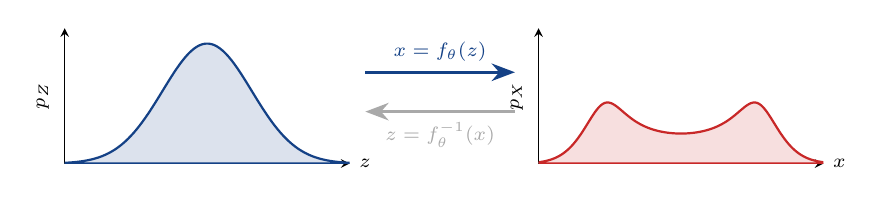
\begin{tikzpicture}
			\begin{axis}[
					name=pz, width=5.2cm, height=3.3cm, axis lines=left,
					xmin=-3.2, xmax=3.2, ymin=0, ymax=0.45,
					xtick=\empty, ytick=\empty, xlabel={$z$}, ylabel={$p_Z$},
					every axis label/.style={font=\scriptsize}, x label style={at={(axis description cs:1,0)}, anchor=west}]
				\addplot[domain=-3.2:3.2, samples=100, thick, FixedBlue, fill=FixedBlue!15] {exp(-x^2/2)/sqrt(2*pi)} \closedcycle;
			\end{axis}
			\begin{axis}[
					at={(pz.east)}, anchor=west, xshift=2.4cm,
					width=5.2cm, height=3.3cm, axis lines=left,
					xmin=-4.5, xmax=4.5, ymin=0, ymax=0.45,
					xtick=\empty, ytick=\empty, xlabel={$x$}, ylabel={$p_X$},
					every axis label/.style={font=\scriptsize}, x label style={at={(axis description cs:1,0)}, anchor=west}]
				\addplot[domain=-3.0:3.0, samples=300, thick, AdaptRed, fill=AdaptRed!15, variable=\t]
				({\t + 1.5*tanh(2*\t)}, {exp(-\t^2/2)/sqrt(2*pi) / (1 + 3/(cosh(2*\t)^2))}) \closedcycle;
			\end{axis}
			\draw[-Stealth, very thick, UCMNavy] ([xshift=0.2cm, yshift=0.3cm]pz.east) -- node[above, font=\scriptsize] {$x = f_\theta(z)$} ++(1.9,0);
			\draw[Stealth-, very thick, mitgray] ([xshift=0.2cm, yshift=-0.2cm]pz.east) -- node[below, font=\scriptsize] {$z = f_\theta^{-1}(x)$} ++(1.9,0);
		\end{tikzpicture}
	\end{center}

	\small Ejemplo: $f(z) = z + 1.5\tanh(2z)$ estira el centro y convierte una gaussiana en una densidad \textbf{bimodal}. La masa de probabilidad se conserva: donde $f$ estira, la densidad baja.

\end{frame}

\begin{frame}[shrink]{F\'ormula de Cambio de Variables}

	\begin{columns}[T]
		\begin{column}{0.48\textwidth}
			\begin{block}{Caso 1D}
				La probabilidad de un intervalo se conserva:
				\[
				p_X(x)\,|dx| = p_Z(z)\,|dz|
				\]
				\[
				\Rightarrow\; p_X(x) = p_Z\big(f^{-1}(x)\big)\left|\frac{d f^{-1}(x)}{dx}\right|
				\]
			\end{block}
		\end{column}

		\begin{column}{0.48\textwidth}
			\begin{center}
				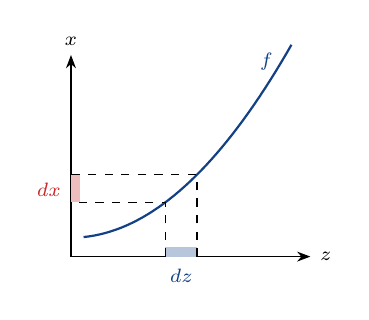
\begin{tikzpicture}[scale=0.8]
					\draw[-Stealth] (0,0) -- (3.8,0) node[right, font=\scriptsize] {$z$};
					\draw[-Stealth] (0,0) -- (0,3.2) node[above, font=\scriptsize] {$x$};
					\draw[thick, UCMNavy, domain=0.2:3.5, samples=40] plot (\x, {0.25*\x*\x + 0.3});
					\fill[FixedBlue!30] (1.5,0) rectangle (2.0,0.15);
					\fill[AdaptRed!30] (0,{0.25*1.5*1.5+0.3}) rectangle (0.15,{0.25*2*2+0.3});
					\draw[dashed] (1.5,0) -- (1.5,{0.25*1.5*1.5+0.3}) -- (0,{0.25*1.5*1.5+0.3});
					\draw[dashed] (2.0,0) -- (2.0,{0.25*2*2+0.3}) -- (0,{0.25*2*2+0.3});
					\node[font=\scriptsize, FixedBlue] at (1.75,-0.3) {$dz$};
					\node[font=\scriptsize, AdaptRed] at (-0.35,{0.25*1.75*1.75+0.3}) {$dx$};
					\node[font=\scriptsize, UCMNavy] at (3.1,3.1) {$f$};
				\end{tikzpicture}
			\end{center}
		\end{column}
	\end{columns}

	\vspace{0.2cm}

	\begin{block}{Caso multivariado ($x, z \in \R^D$)}
		El factor de escala es el valor absoluto del \textbf{determinante del jacobiano}:
	\end{block}

	\formula{
		\[
		\log p_X(x) = \log p_Z\big(f_\theta^{-1}(x)\big) + \log\left|\det \frac{\partial f_\theta^{-1}(x)}{\partial x}\right|
		= \log p_Z(z) - \log\left|\det \frac{\partial f_\theta(z)}{\partial z}\right|
		\]
	}

	\small ¡Verosimilitud \textbf{exacta}! Pero $z$ debe tener la \textbf{misma dimensi\'on} que $x$ (no hay cuello de botella).

\end{frame}

\begin{frame}[shrink]{Componer Transformaciones}

	Una sola $f$ simple no basta. Componemos $K$ capas invertibles:

	\begin{center}
		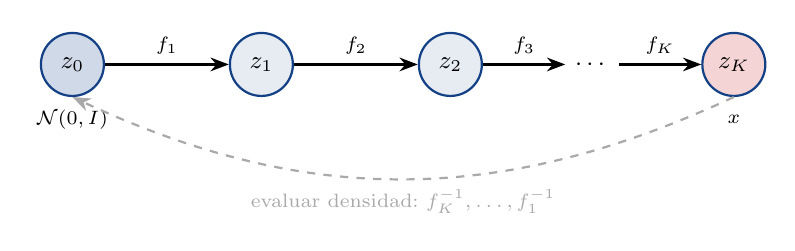
\begin{tikzpicture}[
				st/.style={circle, draw=UCMNavy, thick, fill=UCMNavy!10, minimum size=0.8cm, font=\small},
				arr/.style={-Stealth, thick}]
			\node[st, fill=FixedBlue!20] (z0) at (0,0) {$z_0$};
			\node[st] (z1) at (2.4,0) {$z_1$};
			\node[st] (z2) at (4.8,0) {$z_2$};
			\node[font=\small] (dots) at (6.6,0) {$\cdots$};
			\node[st, fill=AdaptRed!20] (zK) at (8.4,0) {$z_K$};
			\draw[arr] (z0) -- node[above, font=\scriptsize] {$f_1$} (z1);
			\draw[arr] (z1) -- node[above, font=\scriptsize] {$f_2$} (z2);
			\draw[arr] (z2) -- node[above, font=\scriptsize] {$f_3$} (dots);
			\draw[arr] (dots) -- node[above, font=\scriptsize] {$f_K$} (zK);
			\node[font=\scriptsize] at (0,-0.7) {$\mathcal{N}(0,I)$};
			\node[font=\scriptsize] at (8.4,-0.7) {$x$};
			\draw[arr, mitgray, dashed] (zK.south) to[bend left=25] node[below, font=\scriptsize] {evaluar densidad: $f_K^{-1}, \ldots, f_1^{-1}$} (z0.south);
		\end{tikzpicture}
	\end{center}

	\formula{
		\[
		x = f_K \circ \cdots \circ f_1(z_0)
		\qquad\Rightarrow\qquad
		\log p_X(x) = \log p_Z(z_0) - \sum_{k=1}^K \log\left|\det \frac{\partial f_k}{\partial z_{k-1}}\right|
		\]
	}

	\begin{block}{Requisitos de cada capa $f_k$}
		\begin{enumerate}
			\item \textbf{Invertible} (y de preferencia con inversa barata).
			\item Determinante del jacobiano \textbf{barato}: el costo general de $\det$ es $O(D^3)$, inviable para $D \approx 10^5$.
			\item \textbf{Expresiva}: la composici\'on debe poder representar distribuciones complejas.
		\end{enumerate}
	\end{block}

\end{frame}

\begin{frame}[shrink]{Capas de Acoplamiento Af\'in (RealNVP)}

	Dividir $z = (z_A, z_B)$. Una mitad pasa intacta y \textbf{parametriza} la transformaci\'on de la otra:

	\begin{columns}[c]
		\begin{column}{0.48\textwidth}
			\begin{center}
				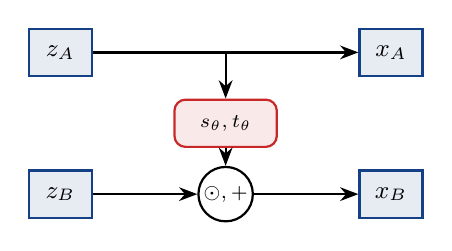
\begin{tikzpicture}[
						v/.style={draw=UCMNavy, thick, fill=UCMNavy!10, minimum width=0.8cm, minimum height=0.6cm, font=\small},
						net/.style={draw=AdaptRed, thick, fill=AdaptRed!10, rounded corners, minimum width=1.3cm, minimum height=0.6cm, font=\scriptsize},
						arr/.style={-Stealth, thick}]
					\node[v] (za) at (0,1.2) {$z_A$};
					\node[v] (zb) at (0,-0.6) {$z_B$};
					\node[v] (xa) at (4.2,1.2) {$x_A$};
					\node[v] (xb) at (4.2,-0.6) {$x_B$};
					\node[net] (st) at (2.1,0.3) {$s_\theta, t_\theta$};
					\node[circle, draw, thick, inner sep=1pt, font=\scriptsize] (op) at (2.1,-0.6) {$\odot,+$};
					\draw[arr] (za) -- (xa);
					\draw[arr] (za) -| (st);
					\draw[arr] (st) -- (op);
					\draw[arr] (zb) -- (op); \draw[arr] (op) -- (xb);
				\end{tikzpicture}
			\end{center}
		\end{column}

		\begin{column}{0.5\textwidth}
			\formula{
				\begin{align*}
					x_A &= z_A\\
					x_B &= z_B \odot \exp\big(\ad{s_\theta(z_A)}\big) + \ad{t_\theta(z_A)}
				\end{align*}
			}
			\small $s_\theta, t_\theta$: redes \textbf{arbitrarias} (CNN, ResNet). Nunca se invierten.
		\end{column}
	\end{columns}

	\vspace{0.2cm}

	\begin{columns}[T]
		\begin{column}{0.5\textwidth}
			\begin{block}{Inversa trivial}
				\small
				\[
				z_A = x_A, \quad z_B = \big(x_B - t_\theta(x_A)\big) \odot \exp\big(-s_\theta(x_A)\big)
				\]
			\end{block}
		\end{column}

		\begin{column}{0.5\textwidth}
			\begin{block}{Jacobiano triangular}
				\small
				\[
				\frac{\partial x}{\partial z} =
				\begin{pmatrix} I & 0 \\ \ast & \mathrm{diag}(e^{s_\theta(z_A)}) \end{pmatrix}
				\]
				\[
				\Rightarrow\;\log|\det| = \textstyle\sum_j s_\theta(z_A)_j
				\]
			\end{block}
		\end{column}
	\end{columns}

	\vspace{0.1cm}

	\small Costo $O(D)$. Se \textbf{alterna} qu\'e mitad se transforma (o se permutan canales) para que todas las variables se mezclen.

\end{frame}

\begin{frame}[shrink]{Flujos Autorregresivos y Otras Arquitecturas}

	\begin{block}{Flujo autorregresivo enmascarado (MAF) e inverso (IAF)}
		Cada dimensi\'on se transforma condicionada en las \textbf{anteriores}:
		\[
		x_i = z_i\, \exp\big(s_i(x_{1:i-1})\big) + t_i(x_{1:i-1})
		\qquad\Rightarrow\qquad
		\text{jacobiano triangular},\; \log|\det| = \textstyle\sum_i s_i
		\]
		\begin{itemize}
			\small
			\item \textbf{MAF}: densidad r\'apida (paralela, con m\'ascaras tipo MADE), muestreo lento ($D$ pasos secuenciales).
			\item \textbf{IAF}: lo contrario. Muestreo r\'apido, densidad lenta. \'Util como $q_\phi$ en un VAE.
		\end{itemize}
	\end{block}

	\vspace{0.2cm}

	\begin{columns}[T]
		\begin{column}{0.5\textwidth}
			\begin{block}{Glow (2018)}
				\small
				\begin{itemize}
					\item ActNorm + convoluci\'on invertible $1\times1$ (permutaci\'on aprendida) + acoplamiento af\'in.
					\item Arquitectura multiescala.
					\item $\log|\det W|$ con descomposici\'on LU.
				\end{itemize}
			\end{block}
		\end{column}

		\begin{column}{0.5\textwidth}
			\begin{block}{Flujos continuos}
				\small
				\begin{itemize}
					\item $\frac{dz(t)}{dt} = v_\theta(z(t), t)$: una ODE neuronal.
					\item $\frac{d \log p(z(t))}{dt} = -\mathrm{tr}\big(\frac{\partial v_\theta}{\partial z}\big)$.
					\item Base del \textbf{flow matching} moderno.
				\end{itemize}
			\end{block}
		\end{column}
	\end{columns}

\end{frame}

\begin{frame}[shrink]{Entrenamiento y Balance de los Flujos}

	\formula{
		\[
		\theta^* = \arg\max_\theta \sum_{i=1}^N \Big[\log p_Z\big(f_\theta^{-1}(x^{(i)})\big) + \log\Big|\det \tfrac{\partial f_\theta^{-1}}{\partial x}\big(x^{(i)}\big)\Big|\Big]
		\]
	}

	\small M\'axima verosimilitud \textbf{exacta} por descenso de gradiente. Se reporta en \textit{bits por dimensi\'on}: $-\log_2 p(x)/D$.

	\vspace{0.3cm}

	\begin{columns}[T]
		\begin{column}{0.5\textwidth}
			\begin{block}{Ventajas}
				\small
				\begin{itemize}
					\item Log-verosimilitud \textbf{exacta}.
					\item Inferencia exacta $z = f^{-1}(x)$.
					\item Muestreo en una pasada (acoplamiento).
					\item Entrenamiento estable.
				\end{itemize}
			\end{block}
		\end{column}

		\begin{column}{0.5\textwidth}
			\begin{alertblock}{Desventajas}
				\small
				\begin{itemize}
					\item $\dim z = \dim x$: sin compresi\'on.
					\item Restricciones arquitect\'onicas $\Rightarrow$ muchos par\'ametros para igualar a otros modelos.
					\item Calidad visual inferior a GAN y difusi\'on.
					\item Topolog\'ia: un homeomorfismo no puede ``romper'' una gaussiana en componentes separados.
				\end{itemize}
			\end{alertblock}
		\end{column}
	\end{columns}

	\vspace{0.2cm}

	\small \textbf{Usos actuales:} estimaci\'on de densidad, detecci\'on de anomal\'ias, distribuciones variacionales flexibles, muestreo en f\'isica (rejillas, mol\'eculas) e inferencia bayesiana amortizada.

\end{frame}

% =================================================================
\section{Redes Generativas Adversarias}

\begin{frame}{GAN: Aprender sin Evaluar la Densidad}

	\textbf{Idea} (Goodfellow et al., 2014): no modelar $p_\theta(x)$ expl\'icitamente; entrenar un generador $G$ contra un \textbf{discriminador} $D$ que intenta distinguir datos reales de falsos.

	\vspace{0.2cm}

	\begin{center}
		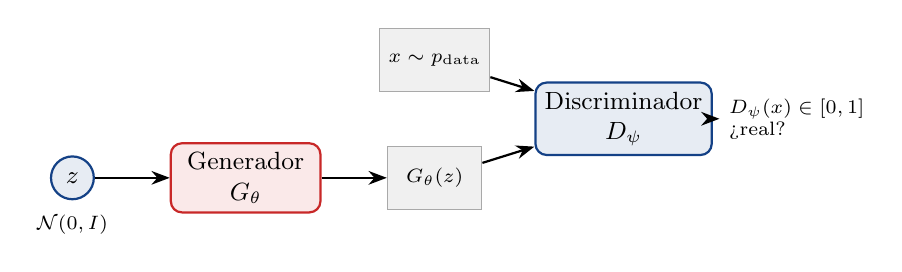
\begin{tikzpicture}[
				box/.style={draw, thick, rounded corners, minimum width=1.9cm, minimum height=0.85cm, align=center, font=\small},
				arr/.style={-Stealth, thick}]
			\node[circle, draw=FixedBlue, thick, fill=FixedBlue!10, font=\small] (z) at (0,0) {$z$};
			\node[box, draw=AdaptRed, fill=AdaptRed!10] (G) at (2.2,0) {Generador\\ $G_\theta$};
			\node[draw=mitgray, fill=LightGray, minimum width=1.2cm, minimum height=0.8cm, font=\scriptsize] (fake) at (4.6,0) {$G_\theta(z)$};
			\node[draw=mitgray, fill=LightGray, minimum width=1.2cm, minimum height=0.8cm, font=\scriptsize] (real) at (4.6,1.5) {$x \sim \pdata$};
			\node[box, draw=UCMNavy, fill=UCMNavy!10] (D) at (7.0,0.75) {Discriminador\\ $D_\psi$};
			\node[font=\scriptsize, align=left] (out) at (9.2,0.75) {$D_\psi(x) \in [0,1]$\\ ¿real?};
			\draw[arr] (z) -- (G); \draw[arr] (G) -- (fake);
			\draw[arr] (fake) -- (D); \draw[arr] (real) -- (D); \draw[arr] (D) -- (out);
			\node[font=\scriptsize] at (0,-0.6) {$\mathcal{N}(0,I)$};
		\end{tikzpicture}
	\end{center}

	\formula{
		\[
		\min_{\theta}\max_{\psi}\; V(G,D) = \E_{x\sim\pdata}\big[\log D_\psi(x)\big] + \E_{z\sim p(z)}\big[\log\big(1 - D_\psi(G_\theta(z))\big)\big]
		\]
	}

	\begin{columns}[T]
		\begin{column}{0.5\textwidth}
			\small $D$ maximiza: clasificador binario con entrop\'ia cruzada.
		\end{column}
		\begin{column}{0.5\textwidth}
			\small $G$ minimiza: enga\~nar a $D$. S\'olo necesita \textbf{muestrear}, nunca evaluar $p_\theta(x)$.
		\end{column}
	\end{columns}

\end{frame}

\begin{frame}{¿Qu\'e Divergencia Minimiza una GAN?}

	Discriminador \'optimo para $G$ fijo: \quad $D^*(x) = \dfrac{\pdata(x)}{\pdata(x) + p_G(x)}$. \quad Sustituyendo en $V$:

	\formula{
		\[
		V(G, D^*) = -\log 4 + 2\,\mathrm{JS}\big(\pdata \,\|\, p_G\big)
		\qquad\Rightarrow\qquad \text{\'optimo global en } p_G = \pdata,\; D^* = \tfrac{1}{2}
		\]
	}

	\small $\mathrm{JS}(p\|q) = \frac{1}{2}\KL\big(p\,\|\,\tfrac{p+q}{2}\big) + \frac{1}{2}\KL\big(q\,\|\,\tfrac{p+q}{2}\big)$: divergencia de Jensen--Shannon, sim\'etrica y acotada.

	\vspace{0.3cm}

	\begin{columns}[T]
		\begin{column}{0.5\textwidth}
			\begin{block}{P\'erdida no saturante (pr\'actica)}
				\small
				Al inicio $D(G(z)) \approx 0$ y $\log(1-D(G(z)))$ tiene gradiente casi nulo. En la pr\'actica $G$ maximiza
				\[
				\E_z\big[\log D_\psi(G_\theta(z))\big]
				\]
			\end{block}
		\end{column}

		\begin{column}{0.5\textwidth}
			\begin{block}{Algoritmo (alternado)}
				\small
				\begin{enumerate}
					\item $k$ pasos de ascenso en $\psi$ con minibatch real + falso.
					\item 1 paso de descenso en $\theta$.
					\item Repetir.
				\end{enumerate}
			\end{block}
		\end{column}
	\end{columns}

\end{frame}

\begin{frame}[shrink]{Dificultades y Mejoras de las GAN}

	\begin{columns}[T]
		\begin{column}{0.5\textwidth}
			\begin{alertblock}{Problemas}
				\small
				\begin{itemize}
					\item \textbf{Colapso de modos}: $G$ produce pocas variantes que enga\~nan a $D$.
					\item \textbf{Inestabilidad}: juego minimax sin garant\'ia de convergencia; oscilaciones.
					\item \textbf{Gradientes que desaparecen}: si los soportes no se solapan, JS es constante ($\log 2$).
					\item Sin verosimilitud: dif\'icil de evaluar (se usa FID).
				\end{itemize}
			\end{alertblock}
		\end{column}

		\begin{column}{0.5\textwidth}
			\begin{block}{Soluciones}
				\small
				\begin{itemize}
					\item \textbf{WGAN}: distancia de Wasserstein (Earth Mover) con cr\'itico 1-Lipschitz:
					\[
					W(\pdata, p_G) = \sup_{\|D\|_L \le 1} \E_{\pdata}[D(x)] - \E_{p_G}[D(x)]
					\]
					\item Penalizaci\'on de gradiente (WGAN-GP), normalizaci\'on espectral.
					\item \textbf{DCGAN}: gu\'ias arquitect\'onicas convolucionales.
					\item \textbf{StyleGAN}: latente mapeado a estilos por capa; fotorrealismo.
				\end{itemize}
			\end{block}
		\end{column}
	\end{columns}

	\vspace{0.3cm}

	\begin{block}{Conexi\'on con la Clase 2.5}
		CycleGAN para \textbf{adaptaci\'on de dominio}: dos generadores $G: A\to B$, $F: B\to A$ con consistencia c\'iclica $\|F(G(x)) - x\|$.
	\end{block}

\end{frame}

% =================================================================
\section{Modelos Basados en Energ\'ia}

\begin{frame}[shrink]{Modelos Basados en Energ\'ia (EBM)}

	\textbf{Idea:} renunciar a la normalizaci\'on. Basta una red escalar $E_\theta : \R^D \to \R$ (la \textbf{energ\'ia}): baja para datos plausibles, alta para el resto.

	\formula{
		\[
		p_\theta(x) = \frac{\exp\big(-E_\theta(x)\big)}{Z_\theta},
		\qquad
		Z_\theta = \int \exp\big(-E_\theta(x)\big)\, dx
		\quad\text{(funci\'on de partici\'on)}
		\]
	}

	\begin{columns}[c]
		\begin{column}{0.55\textwidth}
			\begin{center}
				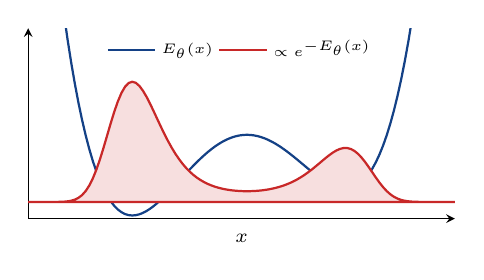
\begin{tikzpicture}
					\begin{axis}[
							width=7cm, height=4.0cm, axis lines=left,
							xmin=-2, xmax=2, ymin=-0.5, ymax=5.2,
							xtick=\empty, ytick=\empty, xlabel={$x$},
							every axis label/.style={font=\scriptsize},
							legend style={font=\tiny, at={(0.5,1.0)}, anchor=north, legend columns=2, draw=none, fill=none}]
						\addplot[domain=-2:2, samples=120, thick, UCMNavy] {2*(x^2-1)^2 + 0.4*x};
						\addplot[domain=-2:2, samples=120, thick, AdaptRed, fill=AdaptRed!15] {2.4*exp(-(2*(x^2-1)^2 + 0.4*x))} \closedcycle;
						\legend{$E_\theta(x)$, $\propto e^{-E_\theta(x)}$}
					\end{axis}
				\end{tikzpicture}
			\end{center}
		\end{column}

		\begin{column}{0.43\textwidth}
			\begin{block}{Ventajas}
				\small
				\begin{itemize}
					\item \textbf{M\'axima flexibilidad}: cualquier arquitectura que produzca un escalar.
					\item Composici\'on: $E = E_1 + E_2$ (producto de expertos).
					\item F\'isica estad\'istica: distribuci\'on de Gibbs/Boltzmann.
				\end{itemize}
			\end{block}
		\end{column}
	\end{columns}

	\vspace{0.1cm}

	\begin{alertblock}{El precio}
		$Z_\theta$ es una integral en $\R^D$: \textbf{intratable}. No podemos evaluar $p_\theta(x)$ ni muestrear directamente.
	\end{alertblock}

\end{frame}

\begin{frame}{Gradiente de la Log-Verosimilitud}

	Aunque $Z_\theta$ es intratable, su gradiente tiene una forma elegante:

	\[
	\nabla_\theta \log Z_\theta = \frac{1}{Z_\theta}\int -\nabla_\theta E_\theta(x)\, e^{-E_\theta(x)}\,dx = -\E_{x\sim p_\theta}\big[\nabla_\theta E_\theta(x)\big]
	\]

	\formula{
		\[
		\nabla_\theta \E_{\pdata}\big[\log p_\theta(x)\big]
		= -\underbrace{\E_{x\sim\pdata}\big[\nabla_\theta E_\theta(x)\big]}_{\text{fase positiva}}
		+ \underbrace{\E_{x'\sim p_\theta}\big[\nabla_\theta E_\theta(x')\big]}_{\text{fase negativa}}
		\]
	}

	\begin{columns}[c]
		\begin{column}{0.48\textwidth}
			\begin{block}{Interpretaci\'on}
				\small
				\begin{itemize}
					\item \textbf{Bajar} la energ\'ia en los datos reales.
					\item \textbf{Subir} la energ\'ia en las muestras del modelo (``alucinaciones'').
					\item Equilibrio: $p_\theta = \pdata$.
				\end{itemize}
			\end{block}
		\end{column}

		\begin{column}{0.5\textwidth}
			\begin{center}
				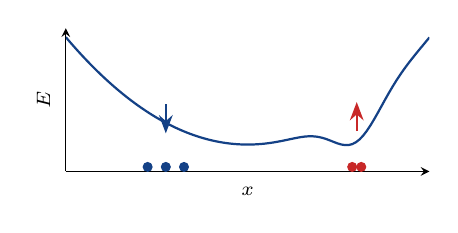
\begin{tikzpicture}
					\begin{axis}[
							width=6.2cm, height=3.4cm, axis lines=left,
							xmin=-2, xmax=2, ymin=0, ymax=3.2,
							xtick=\empty, ytick=\empty, xlabel={$x$}, ylabel={$E$},
							every axis label/.style={font=\scriptsize}]
						\addplot[domain=-2:2, samples=100, thick, UCMNavy] {0.6*x^2 + 0.6 - 0.8*exp(-8*(x-1.2)^2)};
						\addplot[only marks, mark=*, mark size=1.6pt, FixedBlue] coordinates {(-0.9,0.1) (-0.7,0.1) (-1.1,0.1)};
						\addplot[only marks, mark=*, mark size=1.6pt, AdaptRed] coordinates {(1.15,0.1) (1.25,0.1)};
						\draw[-Stealth, thick, FixedBlue] (axis cs:-0.9,1.5) -- (axis cs:-0.9,0.85);
						\draw[-Stealth, thick, AdaptRed] (axis cs:1.2,0.9) -- (axis cs:1.2,1.55);
					\end{axis}
				\end{tikzpicture}
			\end{center}
			\centering\scriptsize \fx{datos}: bajar $E$. \quad \ad{muestras del modelo}: subir $E$.
		\end{column}
	\end{columns}

	\vspace{0.1cm}

	\small El problema se traslada a \textbf{muestrear} $x' \sim p_\theta$.

\end{frame}

\begin{frame}[shrink]{Muestreo con Din\'amica de Langevin}

	\textbf{Observaci\'on clave:} el \textbf{score} $\nabla_x \log p_\theta(x) = -\nabla_x E_\theta(x)$ \textbf{no depende de $Z_\theta$}.

	\formula{
		\[
		x_{k+1} = x_k - \frac{\eta}{2}\,\nabla_x E_\theta(x_k) + \sqrt{\eta}\;\epsilon_k,
		\qquad \epsilon_k \sim \mathcal{N}(0, I)
		\]
	}

	\begin{columns}[c]
		\begin{column}{0.5\textwidth}
			\begin{block}{MCMC por gradiente}
				\small
				\begin{itemize}
					\item Descenso de gradiente sobre la energ\'ia + \textbf{ruido}.
					\item Con $\eta \to 0$ y $K \to \infty$, $x_K \sim p_\theta$.
					\item El ruido evita quedar atrapado en un m\'inimo: explora la distribuci\'on completa.
					\item $\nabla_x E_\theta$ se obtiene con autograd.
				\end{itemize}
			\end{block}
		\end{column}

		\begin{column}{0.48\textwidth}
			\begin{center}
				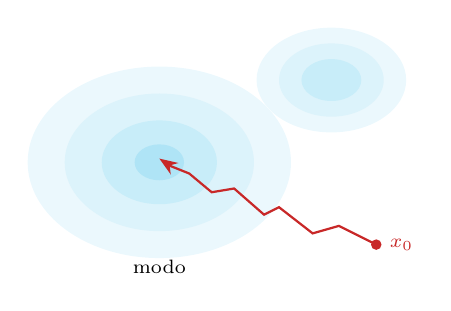
\begin{tikzpicture}[scale=0.95]
					\foreach \r/\c in {1.6/8, 1.15/14, 0.7/22, 0.3/32}{
						\fill[UCMBlue!\c] (1.0,1.3) ellipse ({\r*1.1} and {\r*0.8});
					}
					\foreach \r/\c in {1.0/8, 0.7/14, 0.4/22}{
						\fill[UCMBlue!\c] (3.3,2.4) ellipse ({\r} and {\r*0.7});
					}
					\draw[thick, AdaptRed, -Stealth] (3.9,0.2) -- (3.4,0.45) -- (3.05,0.35) -- (2.6,0.7) -- (2.4,0.6) -- (2.0,0.95) -- (1.7,0.9) -- (1.4,1.15) -- (1.15,1.25) -- (1.0,1.35);
					\fill[AdaptRed] (3.9,0.2) circle (2pt);
					\node[font=\scriptsize, AdaptRed, anchor=west] at (3.95,0.2) {$x_0$};
					\node[font=\scriptsize] at (1.0,-0.1) {modo};
				\end{tikzpicture}
			\end{center}
		\end{column}
	\end{columns}

	\vspace{0.2cm}

	\begin{alertblock}{Costo}
		Cada paso de entrenamiento requiere decenas o cientos de pasos de Langevin: \textbf{lento}, y mezcla mal entre modos separados.
	\end{alertblock}

\end{frame}

\begin{frame}[shrink]{Entrenar un EBM: Divergencia Contrastiva}

	\begin{block}{Algoritmo (Contrastive Divergence / PCD)}
		\small
		\begin{enumerate}
			\item Tomar un minibatch real $\{x^{(i)}\}$.
			\item Generar negativos $\{x'^{(i)}\}$ con $K$ pasos de Langevin, partiendo de:
			\begin{itemize}
				\item los datos (CD-$K$, Hinton 2002), o
				\item un \textbf{buffer de reinicio} con cadenas persistentes (PCD), o ruido uniforme.
			\end{itemize}
			\item Actualizar $\theta$ minimizando la p\'erdida contrastiva:
		\end{enumerate}
	\end{block}

	\formula{
		\[
		\mathcal{L}_{\text{CD}}(\theta) = \frac{1}{B}\sum_{i=1}^B E_\theta\big(x^{(i)}\big) - \frac{1}{B}\sum_{i=1}^B E_\theta\big(\mathrm{sg}[x'^{(i)}]\big) \;+\; \alpha \cdot \text{reg}
		\]
	}

	\small $\mathrm{sg}[\cdot]$: \textit{stop-gradient} (las muestras son constantes). El t\'ermino de regularizaci\'on (p.ej.\ $\alpha(E(x)^2 + E(x')^2)$) evita que las energ\'ias diverjan.

	\vspace{0.1cm}

	\small \textbf{Historia:} m\'aquinas de Boltzmann restringidas (RBM, 2006). \textbf{Moderno:} EBMs con CNN (Du \& Mordatch, 2019) para generaci\'on, inpainting y composici\'on de conceptos.

\end{frame}

\begin{frame}{Alternativas sin Muestreo: Score Matching y NCE}

	\begin{columns}[T]
		\begin{column}{0.5\textwidth}
			\begin{block}{Score Matching (Hyv\"arinen, 2005)}
				\small
				Igualar los \textbf{scores} en vez de las densidades:
				\[
				\tfrac{1}{2}\E_{\pdata}\big\|s_\theta(x) - \nabla_x \log\pdata(x)\big\|^2,
				\]
				con $s_\theta = -\nabla_x E_\theta$. Integrando por partes:
				\[
				\E_{\pdata}\Big[\tfrac{1}{2}\|s_\theta(x)\|^2 + \mathrm{tr}\big(\nabla_x s_\theta(x)\big)\Big]
				\]
				No requiere $Z_\theta$ ni muestras. La traza es cara en alta dimensi\'on.
			\end{block}
		\end{column}

		\begin{column}{0.5\textwidth}
			\begin{block}{Noise-Contrastive Estimation}
				\small
				\begin{itemize}
					\item Clasificar datos reales vs.\ ruido $q(x)$ conocido.
					\item Logit: $\log p_\theta(x) - \log q(x)$, con $\log Z$ como \textbf{par\'ametro aprendido}.
					\item Regresi\'on log\'istica $\Rightarrow$ estimador consistente.
					\item Precursor de las p\'erdidas contrastivas (InfoNCE).
				\end{itemize}
			\end{block}
		\end{column}
	\end{columns}

	\vspace{0.2cm}

	\begin{alertblock}{Denoising Score Matching (Vincent, 2011)}
		Perturbar $\tilde x = x + \sigma\epsilon$ y regresar el ruido:
		$\;\E\big\|s_\theta(\tilde x) + \frac{\tilde x - x}{\sigma^2}\big\|^2$.
		Con muchos niveles de ruido $\sigma_1 > \cdots > \sigma_L$ y Langevin para muestrear $\Rightarrow$ \textbf{modelos de difusi\'on}.
	\end{alertblock}

\end{frame}

\begin{frame}[shrink]{Tu Clasificador es Secretamente un EBM}

	Un clasificador con logits $f_\theta(x) \in \R^K$ define $p_\theta(y\mid x) = \mathrm{softmax}(f_\theta(x))_y$. Reinterpretando los logits como energ\'ias negativas (JEM, Grathwohl et al., 2020):

	\formula{
		\[
		p_\theta(x, y) = \frac{\exp\big(f_\theta(x)[y]\big)}{Z_\theta}
		\quad\Rightarrow\quad
		p_\theta(x) = \frac{\sum_y \exp\big(f_\theta(x)[y]\big)}{Z_\theta},
		\quad E_\theta(x) = -\log\sum_{y}\exp\big(f_\theta(x)[y]\big)
		\]
	}

	\begin{columns}[T]
		\begin{column}{0.5\textwidth}
			\begin{block}{Consecuencias}
				\small
				\begin{itemize}
					\item $p(y\mid x)$ \textbf{no cambia}: $Z_\theta$ se cancela.
					\item Pero la misma red define un modelo generativo de $x$.
					\item Entrenar $\log p(y|x) + \log p(x)$ mejora calibraci\'on y detecci\'on de datos fuera de distribuci\'on.
				\end{itemize}
			\end{block}
		\end{column}

		\begin{column}{0.5\textwidth}
			\begin{block}{Conexi\'on}
				\small
				\begin{itemize}
					\item El softmax es una distribuci\'on de Gibbs sobre clases.
					\item $\mathrm{logsumexp}$ de los logits $\approx$ ``confianza'' del modelo: base de detectores OOD por energ\'ia.
					\item Une las clases discriminativas de la unidad con los modelos generativos.
				\end{itemize}
			\end{block}
		\end{column}
	\end{columns}

\end{frame}

% =================================================================
\section{Comparaci\'on}

\begin{frame}[shrink]{Comparaci\'on de Familias}

	\begin{center}
		\renewcommand{\arraystretch}{1.4}
		\footnotesize\setlength{\tabcolsep}{4pt}
		\begin{tabular}{lcccc}
			\toprule
			& \textbf{VAE} & \textbf{Flujos} & \textbf{GAN} & \textbf{EBM} \\
			\midrule
			Densidad $p_\theta(x)$ & cota (ELBO) & exacta & ninguna & sin normalizar \\
			Muestreo & r\'apido \good & r\'apido \good & r\'apido \good & lento (MCMC) \bad \\
			Calidad de muestras & borrosa \meh & media \meh & alta \good & media/alta \meh \\
			Cobertura de modos & buena \good & buena \good & colapso \bad & buena \good \\
			Latente \'util & compacto \good & $\dim = D$ \meh & sin codificador \meh & no \bad \\
			Estabilidad & alta \good & alta \good & baja \bad & media \meh \\
			Restricci\'on arquitect\'onica & baja & \textbf{alta} & baja & \textbf{ninguna} \\
			\midrule
			Estrategia ante $Z_\theta$ & cota variacional & jacobiano & evitar la densidad & score / MCMC \\
			\bottomrule
		\end{tabular}
	\end{center}

	\vspace{0.2cm}

	\begin{alertblock}{El ``trilema'' generativo}
		Ninguna familia cl\'asica logra a la vez \textbf{alta calidad}, \textbf{cobertura de modos} y \textbf{muestreo r\'apido}. Los modelos de difusi\'on y flow matching sacrifican velocidad para obtener las dos primeras.
	\end{alertblock}

\end{frame}

\begin{frame}{Hacia la Difusi\'on: Lo Que Hereda de Cada Familia}

	\begin{center}
		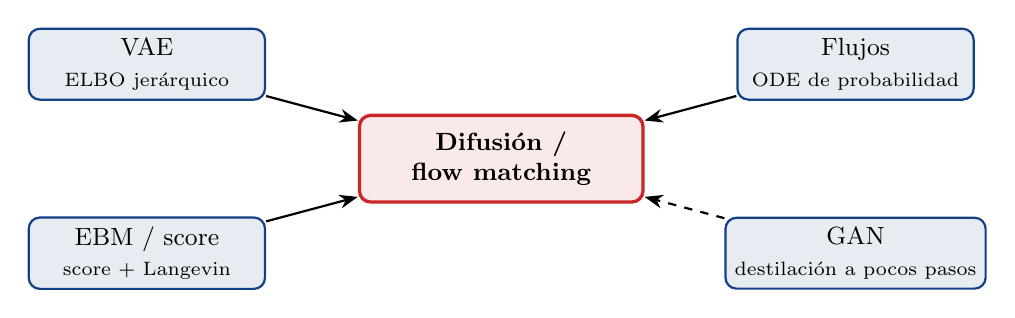
\begin{tikzpicture}[
				fam/.style={draw=UCMNavy, thick, fill=UCMNavy!10, rounded corners, minimum width=3.0cm, minimum height=0.9cm, align=center, font=\small},
				big/.style={draw=AdaptRed, very thick, fill=AdaptRed!10, rounded corners, minimum width=3.6cm, minimum height=1.1cm, align=center, font=\small\bfseries},
				arr/.style={-Stealth, thick}]
			\node[fam] (v) at (-4.5,1.2) {VAE\\ \scriptsize ELBO jer\'arquico};
			\node[fam] (e) at (-4.5,-1.2) {EBM / score\\ \scriptsize score + Langevin};
			\node[fam] (f) at (4.5,1.2) {Flujos\\ \scriptsize ODE de probabilidad};
			\node[fam] (g) at (4.5,-1.2) {GAN\\ \scriptsize destilaci\'on a pocos pasos};
			\node[big] (d) at (0,0) {Difusi\'on /\\ flow matching};
			\draw[arr] (v) -- (d);
			\draw[arr] (e) -- (d);
			\draw[arr] (f) -- (d);
			\draw[arr, dashed] (g) -- (d);
		\end{tikzpicture}
	\end{center}

	\vspace{0.2cm}

	\begin{itemize}
		\item \textbf{VAE}: la difusi\'on es un VAE jer\'arquico con $T$ latentes y codificador fijo (agregar ruido).
		\item \textbf{EBM}: el denoising score matching entrena $s_\theta \approx \nabla_x \log p_\sigma(x)$; se muestrea con Langevin.
		\item \textbf{Flujos}: la ODE de flujo de probabilidad da verosimilitud exacta; flow matching entrena un flujo continuo por regresi\'on.
		\item \textbf{GAN}: discriminadores adversarios para destilar la difusi\'on a pocos pasos.
	\end{itemize}

\end{frame}

% =================================================================
\section{Conclusiones}

\begin{frame}[shrink]{Conclusiones}

	\begin{itemize}
		\item Un modelo generativo aproxima $\pdata$; la m\'axima verosimilitud equivale a minimizar $\KL(\pdata\|p_\theta)$. El obst\'aculo com\'un es la \textbf{normalizaci\'on}.

		\vspace{0.2cm}

		\item \textbf{VAE}: modelo de variable latente entrenado con el ELBO (reconstrucci\'on $-$ KL) y el truco de reparametrizaci\'on. Latente estructurado; muestras algo borrosas.

		\vspace{0.2cm}

		\item \textbf{Flujos normalizantes}: transformaciones invertibles con jacobiano barato (acoplamiento, autorregresivos). Verosimilitud exacta, a costa de restricciones arquitect\'onicas.

		\vspace{0.2cm}

		\item \textbf{GAN}: juego minimax generador--discriminador. Alta calidad visual; inestable y con colapso de modos.

		\vspace{0.2cm}

		\item \textbf{EBM}: densidad no normalizada $e^{-E_\theta(x)}$, m\'axima flexibilidad. Se entrena con fases positiva/negativa (Langevin) o score matching, que conduce a la \textbf{difusi\'on}.
	\end{itemize}

	\vspace{0.3cm}

	\begin{alertblock}{Para el laboratorio}
		Implementar un VAE convolucional en MNIST/Fashion-MNIST: visualizar el espacio latente 2D, interpolar entre d\'igitos y comparar con muestras de un flujo RealNVP en un conjunto 2D (\textit{two moons}).
	\end{alertblock}

\end{frame}

\begin{frame}{Referencias}

	\small
	\begin{itemize}
		\item S.\ J.\ D.\ Prince, \textit{Understanding Deep Learning}, MIT Press, 2023. Caps.\ 14 (no supervisado), 15 (GAN), 16 (flujos normalizantes), 17 (VAE), 18 (difusi\'on). \texttt{udlbook.github.io}
		\item A.\ Torralba, P.\ Isola \& W.\ Freeman, \textit{Foundations of Computer Vision}, MIT Press, 2024. Caps.\ sobre modelos generativos.
		\item D.\ P.\ Kingma \& M.\ Welling, ``Auto-Encoding Variational Bayes'', ICLR 2014.
		\item D.\ J.\ Rezende \& S.\ Mohamed, ``Variational Inference with Normalizing Flows'', ICML 2015.
		\item L.\ Dinh, J.\ Sohl-Dickstein \& S.\ Bengio, ``Density Estimation using Real NVP'', ICLR 2017.
		\item D.\ P.\ Kingma \& P.\ Dhariwal, ``Glow: Generative Flow with Invertible 1x1 Convolutions'', NeurIPS 2018.
		\item I.\ Goodfellow et al., ``Generative Adversarial Nets'', NeurIPS 2014. \quad M.\ Arjovsky et al., ``Wasserstein GAN'', ICML 2017.
		\item Y.\ LeCun et al., ``A Tutorial on Energy-Based Learning'', 2006.
		\item Y.\ Du \& I.\ Mordatch, ``Implicit Generation and Modeling with Energy-Based Models'', NeurIPS 2019.
		\item W.\ Grathwohl et al., ``Your Classifier is Secretly an Energy Based Model'', ICLR 2020.
		\item Y.\ Song \& D.\ P.\ Kingma, ``How to Train Your Energy-Based Models'', arXiv:2101.03288, 2021.
	\end{itemize}

\end{frame}

\end{document}
